\whiteBGstarBegin
\setcounter{section}{0}
\section{Trắc nghiệm}
\begin{enumerate}[label=\bfseries Câu \arabic*:]
	
	\item \mkstar{1}
	
	\cauhoi
	{Hợp lực của hai lực song song cùng chiều $F_1$ và $F_2$ có giá cách hai lực thành phần lần lượt là $d_1$ và $d_2$ tuân theo biểu thức nào sau đây?
		\begin{mcq}(4)
			\item $F_2 d_1 = F_1 d_2$.
			\item $\dfrac{F_2}{F_1} = \dfrac{d_2}{d_1}$.
			\item $\dfrac{F_1}{F_2} = \dfrac{d_1}{d_2}$.
			\item $\dfrac{F_1}{F_2} = \dfrac{d_2}{d_1}$.
		\end{mcq}
	}
	
	\loigiai
	{	\textbf{Đáp án: D.}
		
Hợp lực của hai lực song song cùng chiều $F_1$ và $F_2$ có giá cách hai lực thành phần lần lượt là $d_1$ và $d_2$ tuân theo biểu thức $\dfrac{F_1}{F_2} = \dfrac{d_2}{d_1}$.
	}
	\item \mkstar{1}
	
	\cauhoi
	{Hai lực $\vec F_1$, $\vec F_2$ song song cùng chiều, có độ lớn là $F_1 =\SI{10}{N}$, $F_2=\SI{7}{N}$. Hợp lực của chúng có độ lớn là
		\begin{mcq}(4)
			\item $\SI{20}{N}$.
			\item $\SI{12}{N}$.
			\item $\SI{3}{N}$.
			\item $\SI{17}{N}$.
		\end{mcq}
	}
	
	\loigiai
	{	\textbf{Đáp án: D.}
		
	Hợp lực của hai lực song song cùng chiều có độ lớn:
	$$F=F_1 + F_2 = \SI{17}{N}$$
	}
	
	\item \mkstar{2}
	
	\cauhoi
	{Hai lực song song cùng chiều, có độ lớn $F_1=\SI{5}{N}$, $F_2=\SI{15}{N}$, đặt tại hai đầu một thanh nhẹ (khối lượng không đáng kể). Thanh AB dài $\SI{20}{cm}$. Hợp lực $\vec F = \vec F_1 + \vec F_2$ đặt cách đầu A bao nhiêu và có độ lớn bằng bao nhiêu?
		\begin{mcq}(2)
			\item $\text{OA} = \SI{15}{cm}$, $F=\SI{20}{N}$.
			\item $\text{OA} = \SI{5}{cm}$, $F=\SI{20}{N}$.
			\item $\text{OA} = \SI{15}{cm}$, $F=\SI{10}{N}$.
			\item $\text{OA} = \SI{5}{cm}$, $F=\SI{10}{N}$.
		\end{mcq}
	}
	
	\loigiai
	{	\textbf{Đáp án: A.}
		
	Độ lớn hợp lực:
	$$F=F_1 + F_2 = \SI{20}{N}$$
	
	Áp dụng quy tắc chia trong:
	$$\dfrac{F_1}{F_2} = \dfrac{d_2}{d_1} = \dfrac{\text{AB} - \text{OA}}{\text{OA}} \Rightarrow \text {OA} = \SI{15}{cm}$$
	}
\item \mkstar{2}

\cauhoi
{Một tấm ván AB nặng $\SI{270}{N}$, được bắc qua một con mương. Trọng tâm G của tấm ván cách điểm tựa A một đoạn là $\SI{0.8}{m}$ và cách điểm tựa B là $\SI{1.6}{m}$. Lực mà tấm ván tác dụng lên điểm tựa A là
	\begin{mcq}(4)
		\item $\SI{160}{N}$.
		\item $\SI{180}{N}$.
		\item $\SI{90}{N}$.
		\item $\SI{80}{N}$.
	\end{mcq}
}

\loigiai
{	\textbf{Đáp án: B.}
	
	Độ lớn hợp lực:
	$$F=F_1 + F_2 = \SI{270}{N}$$
	
	Áp dụng quy tắc chia trong:
	$$\dfrac{F_1}{F_2} = \dfrac{d_2}{d_1} = \dfrac{2}{1} \Rightarrow F_1 = \SI{180}{N}$$
}
\item \mkstar{2}

\cauhoi
{Hai bạn Hải và Hùng cùng khiêng một cây gỗ dài $\SI{6}{m}$. Lực nâng của hai bạn đặt ở hai đầu của cây gỗ và đều có phương thẳng đứng. Biết cây gỗ có phương ngang, lực nâng của bạn Hải là $F_1=\SI{60}{N}$ và bạn Hùng là $F_2=\SI{30}{N}$. Trọng tâm của cây gỗ cách bạn Hải một đoạn bằng
	\begin{mcq}(4)
		\item $\SI{2}{m}$.
		\item $\SI{3}{m}$.
		\item $\SI{1.5}{m}$.
		\item $\SI{4}{m}$.
	\end{mcq}
}

\loigiai
{	\textbf{Đáp án: A.}
	
Ta có:
$$d_1+d_2=\SI{6}{m}$$

Áp dụng quy tắc chia trong:
$$\dfrac{F_1}{F_2} = \dfrac{d_2}{d_1} = \dfrac{2}{1} \Rightarrow d_1 = \SI{2}{cm}$$
}
\item \mkstar{2}

\cauhoi
{Một tấm ván nặng $\SI{240}{N}$ được bắc qua một con mương. Trọng tâm của tấm ván cách điểm tựa A $\SI{2.4}{m}$ và cách điểm tựa B $\SI{1.2}{m}$. Hỏi lực mà tấm ván tác dụng lên điểm A bằng bao nhiêu?
	\begin{center}
		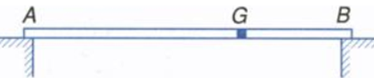
\includegraphics[scale=0.8]{../figs/VN10-2021-PH-TP022-6.png}
	\end{center}
	\begin{mcq}(4)
		\item $\SI{160}{N}$.
		\item $\SI{80}{N}$.
		\item $\SI{120}{N}$.
		\item $\SI{60}{N}$.
	\end{mcq}
}

\loigiai
{	\textbf{Đáp án: B.}
	
	Ta có:
	$$P_\text A + P_\text B=\SI{240}{N}$$
	
	Áp dụng quy tắc chia trong:
	$$\dfrac{P_\text{A}}{P_\text{B}} = \dfrac{d_2}{d_1} = \dfrac{1}{2} \Rightarrow P_\text{A} = \SI{80}{N}$$
}
	\item \mkstar{3}
	
	\cauhoi
	{Đặt tại hai đầu một thanh AB dài $\SI{40}{cm}$ hai lực song song cùng chiều và vuông góc với AB. Hợp lực $\vec F$ của hai lực đặt tại O cách A một đoạn $\SI{25}{cm}$ và có độ lớn $\SI{10}{N}$. Độ lớn của $\vec F_1$ bằng
		\begin{mcq}(4)
			\item $\SI{2.25}{N}$.
			\item $\SI{8.25}{N}$.
			\item $\SI{3.75}{N}$.
			\item $\SI{6.25}{N}$.
		\end{mcq}
	}
	
	\loigiai
	{	\textbf{Đáp án: C.}	
		
	
	Áp dụng quy tắc chia trong:
	$$\dfrac{F_1}{F_2} = \dfrac{d_2}{d_1} = \dfrac{\text{AB} - \text{OA}}{\text{OA}} = \dfrac{3}{5} \Rightarrow F_2 = \dfrac{5}{3}F_1$$
	
		Độ lớn hợp lực:
	$$F=F_1 + F_2 =F_1 + \dfrac{5}{3}F_1= \SI{10}{N} \Rightarrow F_1 = \SI{3.75}{N}$$
	}
	
	
	
	\item \mkstar{3}
	
	\cauhoi
	{Một người đang quẩy trên vai một chiếc bị có trọng lượng $\SI{50}{N}$. Chiếc bị buộc ở một đầu gậy cách vai $\SI{60}{cm}$. Tay người giữ ở đầu kia cách vai $\SI{30}{cm}$. Bỏ qua trọng lượng của gậy. Lực giữ của tay là
		\begin{mcq}(4)
			\item $\SI{50}{N}$.
			\item $\SI{75}{N}$.
			\item $\SI{100}{N}$.
			\item $\SI{150}{N}$.
		\end{mcq}
	}
	
	\loigiai
	{	\textbf{Đáp án: C.}
		
		\begin{center}
			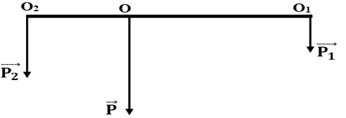
\includegraphics[scale=1]{../figs/VN10-2021-PH-TP022-3.png}
		\end{center}
		
	Gọi lực giữ của tay là $\vec P_2$, trọng lượng của bị là $\vec P_1$.
	
	Ta có:
	$$\dfrac{P_2}{P_1} = \dfrac{d_1}{d_2} = 2 \Rightarrow P_2 = 2 P_1 = \SI{100}{N}$$
	}
	
	\item \mkstar{3}
	
	\cauhoi
	{Hai người cầm hai đầu của một chiếc gậy để khiêng một vật nặng, gậy có trọng lượng không đáng kể, dài $\SI{1.4}{m}$. Vật có trọng lượng $\SI{700}{N}$ được treo vào điểm C cách đầu A $\SI{0.6}{m}$. Hỏi người ở B chịu một lực bằng bao nhiêu?
		\begin{mcq}(4)
			\item $\SI{200}{N}$.
			\item $\SI{300}{N}$.
			\item $\SI{400}{N}$.
			\item $\SI{600}{N}$.
		\end{mcq}
	}
	
	\loigiai
	{	\textbf{Đáp án: B.}
		
	Ta có: $P=\SI{700}{N}$, $\text{AC} = \SI{0.6}{m}$, $\text{BC} = \SI{0.8}{m}$.
	
	Áp dụng quy tắc tổng hợp hai lực song song cùng chiều:
	\begin{cases}
		P=P_1+P_2=\SI{700}{N} \\
		\dfrac{P_1}{P_2} = \dfrac{\text{AC}}{\text{BC}} = \dfrac{4}{3}
	\end{cases}
	
	Tính được:
	\begin{cases}
		P_1 = \SI{400}{N} \\
		P_2 = \SI{300}{N}
	\end{cases}

	Vậy người B chịu một lực là $P_1=\SI{300}{N}$.
	}
	\item \mkstar{3}

\cauhoi
{Hãy xác định trọng tâm của một bản phẳng mỏng, đồng chất, hình chữ nhật dài $\SI{12}{cm}$, rộng $\SI{6}{cm}$, bị cắt mất một phần hình vuông có cạnh $\SI{3}{cm}$ ở một góc (hình vẽ).
	\begin{center}
		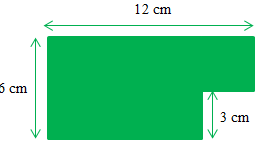
\includegraphics[scale=1]{../figs//VN10-2021-PH-TP022-4.png}
	\end{center}
Gọi $\text O_1$ là tâm của hình chữ nhật, $\text O_2$ là tâm của hình vuông. Chọn phát biểu đúng.
	\begin{mcq}
		\item Trọng tâm G nằm trên đường nối $\text O_1$ và $\text O_2$ và cách $\text O_1$ một đoạn $\SI{0.88}{cm}$.
		\item Trọng tâm G nằm trên đường nối $\text O_1$ và $\text O_2$ và cách $\text O_1$ một đoạn $\SI{5.3}{cm}$.
		\item Trọng tâm G nằm trên đường vuông góc với đường nối $\text O_1$ và $\text O_2$ và cách $\text O_1$ một đoạn $\SI{0.88}{cm}$.
		\item Trọng tâm G nằm trên đường vuông góc với đường nối $\text O_1$ và $\text O_2$ và cách $\text O_1$ một đoạn $\SI{5.3}{cm}$.
	\end{mcq}
}

\loigiai
{	\textbf{Đáp án: A.}
	
		\begin{center}
		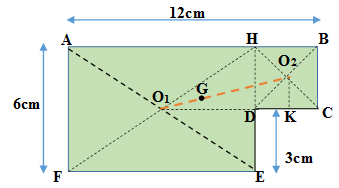
\includegraphics[scale=1]{../figs//VN10-2021-PH-TP022-5.png}
	\end{center}

	Vì các bản đồng chất, phẳng mỏng đều nên tỉ lệ diện tích bằng tỉ lệ về trọng lượng:
	$$\dfrac{P_1}{P_2} = \dfrac{S_\text{AEHF}}{S_\text{HBCD}} = \dfrac{6 \cdot 9}{3 \cdot 3} = 6$$
	
	Gọi G là trọng tâm của cả bản phẳng. G phải nằm trên đoạn thẳng $\text O_1 \text O_2$, trong đó $\text O_1$ là trọng tâm của bản $\text{AEHF}$, $\text O_2$ là trọng tâm của bản $\text{HBCD}$.
	
	Ta có:
	$$\dfrac{P_1}{P_2} = \dfrac{\text{GO}_2}{\text{GO}_1} = 6 \Rightarrow 6 \text{GO}_1 - \text{GO}_2 = 0$$
	
	Xét tam giác vuông $\text O_1 \text O_2 \text K$, ta có:
	$$\text O_1 \text O_2 = \sqrt{(\text O_2 \text K)^2 + (\text O_1 \text K)^2} = \sqrt{1,5^2 + 6^2} = 6,18 \Rightarrow \text G \text O_1 + \text G \text O_2 =6,18$$
	
	Giải hệ, tìm được $\text G \text O_1 = \SI{0.88}{cm}$.
	
	Vậy trọng tâm G nằm trên đường nối $\text O_1$ và $\text O_2$ và cách $\text O_1$ một đoạn $\SI{0.88}{cm}$.
}	
\end{enumerate}

\whiteBGstarEnd

\loigiai
{
	\begin{center}
		\textbf{BẢNG ĐÁP ÁN}
	\end{center}
	\begin{center}
		\begin{tabular}{|m{2.8em}|m{2.8em}|m{2.8em}|m{2.8em}|m{2.8em}|m{2.8em}|m{2.8em}|m{2.8em}|m{2.8em}|m{2.8em}|}
			\hline
			1.D  & 2.D  & 3.A  & 4.B  & 5.A  & 6.B & 7.C & 8.C & 9.B & 10.A  \\
			\hline
			
		\end{tabular}
	\end{center}
}
\section{Tự luận}
\begin{enumerate}[label=\bfseries Câu \arabic*:]
	\item \mkstar{1}
	
	\cauhoi{
		Phát biểu quy tắc tổng hợp hai lực song song cùng chiều.
	}
	
	\loigiai{
		Hợp lực của hai lực song song cùng chiều là một lực song song cùng chiều và có độ lớn bằng tổng độ lớn của hai lực ấy.
		$$\vec F = \vec F_1 + \vec F_2$$
		
		Giá của hợp lực chia khoảng cách giữa hai giá của hai lực song song thành những đoạn tỉ lệ với độ lớn của hai lực ấy.
		$$\dfrac{F_1}{F_2} = \dfrac{d_2}{d_1}$$
	}
	
	\item \mkstar{2}
	
	\cauhoi
	{Một người gánh một thùng gạo nặng $\SI{300}{N}$ và một thùng gỗ nặng $\SI{200}{N}$. Đòn gánh dài $\SI{1}{m}$. Hỏi vai người đó phải đặt ở điểm nào, chịu một lực bằng bao nhiêu? Bỏ qua trọng lượng của đòn gánh.
	}
	
	\loigiai
	{
		Áp dụng quy tắc hợp lực song song cùng chiều, ta có:
		$$P = P_1 + P_2 = \SI{500}{N}$$
		
		$$\dfrac{P_1}{P_2} = \dfrac{\text{OB}}{\text{OA}} = \dfrac{3}{2}$$
		
		Ta có hệ phương trình:
		\begin{cases}
			3 \text{OA} - 2 \text{OB} = 0 \\
			\text{OA} + \text{OB} = 100
		\end{cases}
	Suy ra:
	\begin{cases}
		\text{OA} = \SI{40}{cm} \\
		\text{OB} = \SI{60}{cm}
	\end{cases}
	}
	\item \mkstar{3}
	
	\cauhoi
	{Một tấm ván nặng $\SI{240}{N}$ được bắc qua một con mương. Trọng tâm của tấm ván cách điểm tựa A $\SI{2.4}{m}$ và cách điểm tựa B $\SI{1.2}{m}$. Hỏi lực mà tấm ván tác dụng lên điểm tựa B bằng bao nhiêu?
	}
	
	\loigiai
	{Ta có:
		\begin{cases}
			P_\text{A} + P_\text{B} = \SI{240}{N} \\
			\dfrac{P_\text{A}}{P_\text{B}} = \dfrac{\text{GB}}{\text{GA}} = \dfrac{1}{2}
		\end{cases}
	
	Suy ra:
			\begin{cases}
		P_\text{A} + P_\text{B} = \SI{240}{N} \\
		P_\text{B} = 2 P_\text{A}
	\end{cases}

	Suy ra $P_\text{B} = \SI{160}{N}$.
	}
	\item \mkstar{4}
	
	\cauhoi
	{Một thanh cứng AB có khối lượng không đáng kể, dài $\SI{1}{m}$, được treo nằm ở hai đầu AB nhờ hai lò xo thẳng đứng có chiều dài tự nhiên bằng nhau và có độ cứng lần lượt là $k_1=\SI{90}{N/m}$ và $k_2=\SI{60}{N/m}$. Để thanh vẫn nằm ngang phải treo một vật nặng vào điểm C cách A một khoảng là bao nhiêu?
	}
	
	\loigiai
	{Lực đàn hồi: $F=k \Delta l \Rightarrow \Delta l = \dfrac{F}{k}$.
		
	Hai lò xo phải dãn như nhau:
	$$\Delta l_1 = \Delta l_2 \Rightarrow \dfrac{F_1}{k_1} = \dfrac{F_2}{k_2} \Rightarrow \dfrac{F_1}{F_2} = \dfrac{k_1}{k_2} = 1,5$$
	
	Mặt khác, $\dfrac{F_1}{F_2} = \dfrac{\text{CB}}{\text{CA}} \Rightarrow \text{CB} = 1,5 \text{CA}$.
	
	Kết hợp với $\text{CA} + \text{CB} = \SI{100}{cm}$.
	
	Tìm được $\text{CA} = \SI{40}{cm}$, $\text{CB} = \SI{60}{cm}$.
	}
	\item \mkstar{4}
	
	\cauhoi
	{Một thanh AB dài $\SI{1}{m}$ khối lượng $\SI{5}{kg}$ được đặt nằm ngang lên hai giá đỡ tại A và B. Người ta móc vào điểm C của thanh ($\textrm{AC}=\SI{60}{cm}$) một vật nặng có khối lượng $\SI{10}{kg}$. Lấy $g=\SI[parse-numbers=false]{10}{m/s^2}$, lực nén trên hai giá đỡ là bao nhiêu? 
	%%%%%%%%%
	\begin{center}
		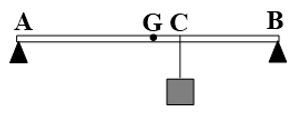
\includegraphics[scale=1]{../figs/VN10-2021-PH-TP022-1.png}
	\end{center}
	}
	
	\loigiai
	{ Đầu tiên, ta phân tích các lực tác dụng lên thanh như trong hình dưới. 
		\begin{center}
			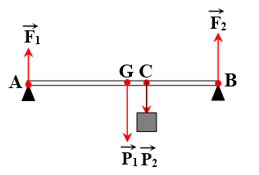
\includegraphics[scale=1]{../figs/VN10-2021-PH-TP022-2.png}
		\end{center}
		%%%%
		Ngoài trọng lượng $\vec{P}_2$ của vật nặng, ta còn xét thêm trọng lượng $\vec{P}_1$ của thanh. Vì thanh đang ở vị trí cân bằng nên theo quy tắc tổng hợp các lực song song:
		\begin{equation*}
			\vec{F}_1+\vec{F}_2=\vec{P}_1+\vec{P}_2=\vec{P},
		\end{equation*}
		với $\vec{P}$ là tổng hợp lực của hai trọng lượng, 
		%
		và độ lớn của chúng có liên hệ 
		\begin{equation*}
			P=F_1+F_2=P_1+P_2 = m_1\cdot g + m_2\cdot g = \SI{150}{N}. 
		\end{equation*}
		%
		Gọi $d_1$ và $d_2$ là khoảng cách từ giá của các lực $\vec{P}_1$ và $\vec{P}_2$ đến giá của tổng hợp lực $\vec{P}$:
		\begin{equation*}
			d_1+d_2=\textrm{GC}=\textrm{AC}-\textrm{AG} = \SI{60}{cm}-\dfrac{1}{2}\SI{100}{cm}=\SI{10}{cm}.\tag{1} 
		\end{equation*}
		Áp dụng quy tắc chia trong cho hai trọng lượng, ta có
		\begin{equation*}
			\dfrac{d_2}{d_1}=\dfrac{P_1}{P_2}=\dfrac{1}{2}
			\Rightarrow
			d_1-2d_2=0. \tag{2}
		\end{equation*}
		Từ (1) và (2) ta có $d_1=\SI[parse-numbers=false]{\dfrac{20}{3}}{cm}$ và $d_1=\SI[parse-numbers=false]{\dfrac{10}{3}}{cm}$. 
		Từ đó, ta tính được khoảng cách $d'_1$ và $d'_2$ từ giá của $\vec{F}_1$ và $\vec{F}_2$ đến giá của $\vec{P}$ như sau:
		\begin{align*}
			d'_1&=\textrm{AG}+d_1=\SI[parse-numbers=false]{\dfrac{170}{3}}{cm},\\
			d'_2&=\textrm{BC}+d_2=\SI[parse-numbers=false]{\dfrac{130}{3}}{cm}.
		\end{align*}
		%%
		Áp dụng quy tắc chia trong cho hai lực căng dây, ta có liên hệ:
		\begin{align*}
			\dfrac{F_1}{F_2}=\dfrac{d'_2}{d'_1}
			=
			\dfrac{\SI[parse-numbers=false]{\dfrac{130}{3}}{cm}}{\SI[parse-numbers=false]{\dfrac{170}{3}}{cm}}
			\Rightarrow
			17F_1-13F_2=0\ (3). 
		\end{align*}
		Từ (1) và (3), ta tính được độ lớn các lực căng dây: $F_1=\SI{65}{N}$ và $F_2=\SI{85}{N}$. 
	}
\end{enumerate}